%! Author = opiwa
%! Date = 04.01.2023

\clearpage
\subsection{Mitigation}\label{subsec:mitigation}
Da es sich bei Log4Shell um einen 0-day handelt, war es besonders wichtig, in der Zeit bis alle Dependencies gepatcht sind, Möglichkeiten der Mitigierung zu finden.

Für eine bessere Übersicht, an welchen Stellen Log4Shell mitigiert werden kann, hat die Schweizer Regierung eine übersichtliche Grafik erstellt.\footfullcite{schweizGov}

\begin{figure}[!htb]\label{fig:log4jattackgraphic}
    \begin{center}
        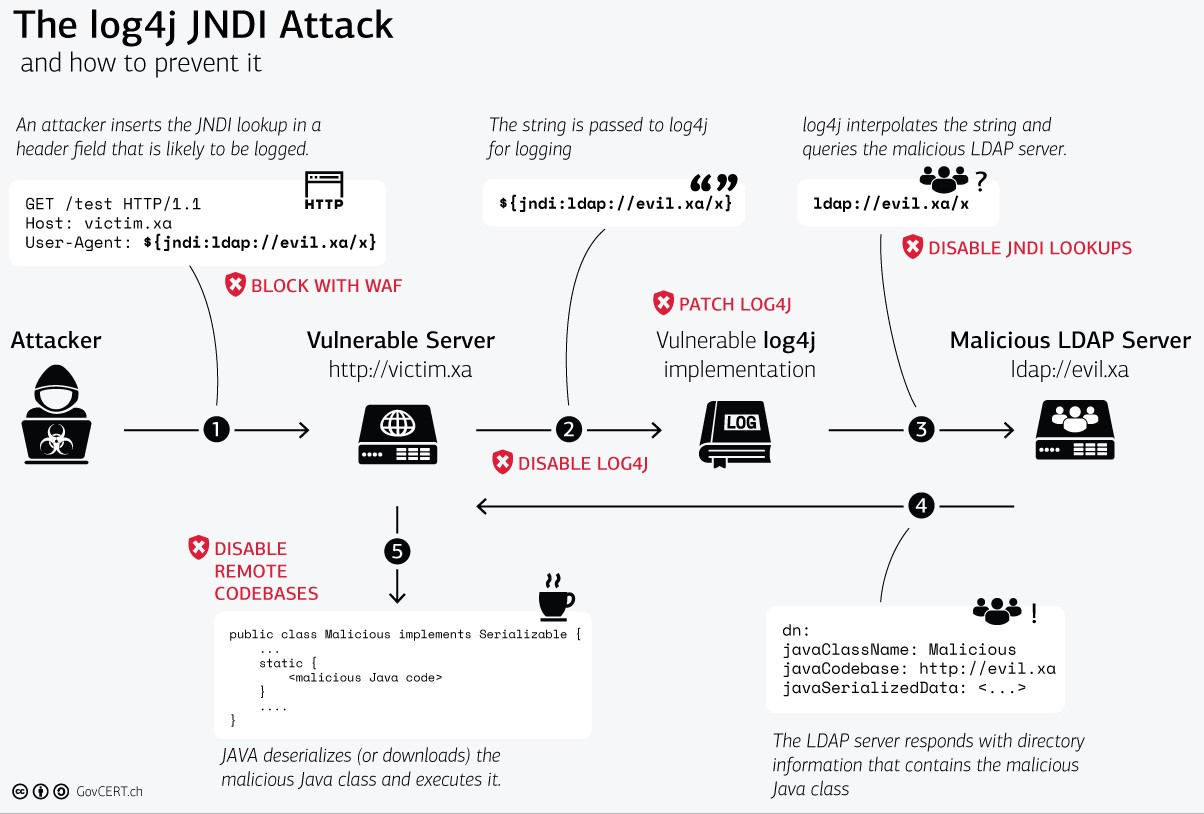
\includegraphics[width=\textwidth]{images/log4j_attack}
    \end{center}
    \caption{Log4j Attack and Mitigations}
\end{figure}

Eine der schnellsten Möglichkeiten Log4Shell zu mitigieren, ist es
\\ \verb|org.apache.logging.log4j.core.lookup.JndiLookup|\\
aus dem classpath zu entfernen.\footfullcite{redditThread}

Dieser Schritt führt dazu, dass der Logger keine \gls{jndi} Lookups mehr durchführen kann, wodurch der Angriffsvektor komplett wegfällt.
Da \verb|JndiLookup| allerdings ein wesentlicher Bestandteil des Featuresets von Log4j ist, ist dieser Schritt - obwohl effektiv - nur eine Kurzzeitlösung.

Das Problem dieser Lösung ist allerdings, dass dadurch nur die \gls{rce} Sicherheitslücke in CVE-2021-44228 mitigiert wird.
Es ist allerdings weiterhin möglich, dass Benutzereingaben evaluiert werden und zu StackOverflows führen oder private Daten preisgeben.\footfullcite{log4jSecurity}
Daher ist es trotz der Mitigierungsmöglichkeiten wichtig, die Sicherheitspatches so früh wie möglich aufzuspielen oder einen \gls{jndi} Live patch einzuspielen.
